\documentclass{article_saj}
\usepackage{graphicx,saj,multicol,subeqnarray}
\usepackage{float}
\usepackage{xcolor}
\usepackage{widetext}
\usepackage{url}
\usepackage{bm}
\usepackage{tikz} % for checkmark
\usepackage{pifont} % for xmark
\usepackage{amsfonts}
\usepackage{amssymb}
\usepackage{amsmath,upgreek}
\usepackage{titlesec}
\usepackage{fancyhdr}
\usepackage{caption}
\usepackage[english]{babel}
\usepackage[nottoc]{tocbibind}
\usepackage[skip=\medskipamount]{parskip}
\def\tg{\mathop{\rm tg}\nolimits}
\def\arctg{\mathop{\rm arctg}\nolimits}

\def\point#1{\hbox{\setbox7=\hbox to0.6em{\hfil.\hfil}%
\setbox8=\hbox to0.5em{\hfil$^{#1}$\hfil}%
\box7\kern-0.5em\box8}}

\def\pointmin#1{\hbox{\setbox2=\hbox to0.8em{\hfil.\hfil}%
\setbox3=\hbox to0.6em{\hfil$^{#1}$\hfil}%
\box2\kern-.7em\box3}}

%for non integer numbers for years, days, hours, minutes and seconds

\def\yyy{\point{\mathrm{y}}}
\def\ddd{\point{\mathrm{d}}}
\def\hhh{\point{\mathrm{h}}}
\def\mmm{\pointmin{\mathrm{m}}\kern.15em}
\def\sss{\point{\mathrm{s}}}

%for non integer numbers for arc degrees, arc minutes and arc seconds

\def\oo{\point{\circ}}
\def\lll{\point{\prime}}
\def\uu{\point{\prime\prime}}

%for integer numbers for arc degrees, arc minutes and arc seconds

\def\OO{$^\circ$}
\def\LLL{$^\prime$}
\def\UU{$^{\prime\prime}$}
 

\pagestyle{myheadings}
\titlelabel{\thetitle.\quad}
\definecolor{xlinkcolor}{cmyk}{1,0.6,0,0}
\usepackage[bookmarks=false,         % show bookmarks bar?
     pdfnewwindow=true,      % links in new window
     colorlinks=true,    % false: boxed links; true: colored links
     linkcolor=xlinkcolor,     % color of internal links
     citecolor=xlinkcolor,     % color of links to bibliography
     filecolor=xlinkcolor,  % color of file links
     urlcolor=xlinkcolor,      % color of external links
final=true
]{hyperref}

\def\papertype{\ \hfill\ Editorial}

\def\udc{52}
\setcounter{publno}{200}
\setcounter{publyear}{2020}
\setcounter{page}{1}
\setcounter{firstpage}{1}
\setcounter{lastpage}{5}
\setcounter{footnote}{0}
\renewcommand{\thefootnote}{\fnsymbol{footnote}}

\begin{document}

\pagestyle{fancy}
\fancyhead{}
\renewcommand{\headheight}{0pt}
\renewcommand{\headrulewidth}{0pt}

\parindent=0cm
\baselineskip=3.8truemm
\columnsep=.75truecm

\newenvironment{lefteqnarray}{\arraycolsep=0pt\begin{eqnarray}}
{\end{eqnarray}\protect\aftergroup\ignorespaces}
\newenvironment{lefteqnarray*}{\arraycolsep=0pt\begin{eqnarray*}}
{\end{eqnarray*}\protect\aftergroup\ignorespaces}
\newenvironment{leftsubeqnarray}{\arraycolsep=0pt\begin{subeqnarray}}
{\end{subeqnarray}\protect\aftergroup\ignorespaces}

\begin{strip}
{\ }
\vskip-5cm
{\ }

\title{Single Pulse Timing Study of Pulsars and its Relationship with Pulse Jitter}

\authors{Aditya Gupta}

\vskip2mm
\begin{center}
BTech in Mathematics and Computing, Indian Institute of Science, Bengaluru  
\end{center}

\vskip1mm
\begin{center}
  Email: \textit{adityapg@iisc.ac.in}
\end{center}

\vskip3mm
\noindent This is a preliminary report of my work for the NIUS Astronomy project under the guidance of Prof. Bhal Chandra Joshi. This report contains a summary of the research I have done about radio astronomy and pulsars. It also contains the methodology and results of the initial analysis that I performed on data from the pulsar B1133+16. 

\end{strip}
\tenrm

\section{INTRODUCTION}
In 1933, Karl Jansky discovered radio wave emissions from the Sagittarius constellation in the Milky Way. This monumental discovery opened the door for modern radio astronomy. 

Radio astronomy is the study of the universe at radio frequencies. While the waves emitted at these frequencies are not visible to the naked eye, they are extremely important for the study of several astronomical phenomenon. Celestial objects which emit strong radio waves are called radio sources. Neutron stars, pulsars, radio galaxies and black holes are some of the most prominent radio sources. The background radiation left over after the Big Bang, called the Cosmic Microwave Background (CMB), is also an important radio source which helps us study the origins of the universe.


\section{RADIO WAVES}
For the most part, radio waves can be treated like regular electromagnetic waves. Electromagnetic emissions from a blackbody follow the Planck distribution, which is given by the equation:
\begin{equation}
  I_{\nu} = \frac{2h\nu^3}{c^2}\frac{1}{e^{h\nu / kT}-1}
\end{equation}
where $I_{\nu}$ is the intensity of the radiation, $\nu$ is the frequency of the radiation, $h$ is Planck's constant, $c$ is the speed of light, $k$ is the Boltzmann constant and $T$ is the temperature of the blackbody. This formula is valid for all frequencies of radiation, including radio waves. 

We can find the temperature of a blackbody by fitting a Planck curve on the entire spectrum. Alternatively, we can use the Wien's displacement law, which states that the peak of the Planck curve is inversely proportional to the temperature of the blackbody. This is given by the equation:
\begin{equation}
  \lambda_{\text{max}} = \frac{b}{T}
\end{equation}
where $\lambda_{\text{max}}$ is the wavelength at which the intensity of the radiation is maximum, $b$ is Wien's displacement constant and $T$ is the temperature of the blackbody.

However for radio astronomy, we deal with waves of relatively low frequencies, where quantum effects can be ignored. At these frequencies, we can use a simpler version of the Planck distribution, called the Rayleigh-Jeans approximation, to calculate the temperature. It is given by:
\begin{equation}
  I_{\nu} = \frac{2\nu^2kT}{c^2} = \frac{2 kT}{\lambda^2}
\end{equation}
It is important to note that the temperature obtained from these methods is only valid if we are measuring thermal radiation. We refer to this as the \textit{brightness temperature} of the blackbody. This becomes relevant when we study radio emissions from celestial objects as not all radio emissions are thermal in nature. Broadly speaking, we can categorise radio emissions into two types - thermal and non-thermal emissions.

\subsection{Thermal emissions}
Thermal emissions are the result of ion interactions within the object. Their intensity vs frequency curve follows the Planck distribution. These are directly related to the brightness temperature of the body. This type of radiation is known as free-free, or \textit {bremsstrahlung} radiation. The simplest example for thermal radio emissions is from the CMB, which shows that its temperature is around 2.72 K. It is a broadband radiation, meaning it is emitted over a wide range of frequencies. We generally observe these emissions at the centimeter wavelengths.

\subsection{Non-thermal emissions}
Apart from thermal radio emissions, we also observe strong radiation in the metre wavelength range. This is not a result of the brightness temperature of the body. Instead, it is caused by some other phenomenon inside the body which is not related to its temperature. These are called non thermal emissions. Most of the strong sources of radio emissions, such as supernova remenants and pulsars are non thermal in nature. 

Radio emissions give us a lot more visibility of the cosmos compared to standard optical emissions. Radio waves can easily penetrate dust and gas which generally absorbs and scatters radiation in most other wavebands. This allows us to study the structure of galaxies and molecular clouds in great detail.


\section{MEASURING THE SIGNALS}
To measure the radiation coming from a source, we use an antenna. An antenna receives the electromagnetic waves and converts them into electrical signals. The power received by the antenna depends on its collecting area. 

For a source of flux $S$, its flux density or specific flux at a frequency $\nu$ is given by $S_{\nu}$. Using this, we define the power spectral density $P_{\nu}$ as:
\begin{equation}
  P_{\nu} = S_{\nu}A_{\text{eff}}
\end{equation}

We also define the specific brightness $B_{\nu}$ as:
\begin{equation}
  B_{\nu} = \frac{S_{\nu}}{\Omega_{\text{source}}}
\end{equation}

Using these measures, we can define brightness temperature of a source to be $T_B$ if a hypothetical blackbody of physical temperature $T_B$ would produce the same specific intensity $I_{\nu}$ as the source. However, the specific intensity can be equated to the specific brightness, which gives us:
\begin{equation}
  B_{\nu} = \frac{2 kT_B}{\lambda^2}
\end{equation}
The brightness temperature should not be confused with the physical temperature of the source. Some pulsars have brightness temperatures of $10^{30}$ K, which is much higher than the physical temperature of any known object. This is because their radiation is non-thermal in nature.


\section{NOISE IN THE SIGNAL}
To study the characterisitics of any object, we try to measure the signal coming from it. However, the signal we receive generally contains additional signals which are not emitted by the source we are studying. These extra signals which are not coming directly from the source are called noise. This unwanted noise which comes with the signal can disrupt our measurements. To perform accurate measurements, we need to collect data with a high signal-to-noise ratio.

Noise can be of various types and can be caused by a variety of sources.

\subsection{Random noise}
All natural signals, when incident on an antenna, produce some amount of random variations in the intensity of the signal. These variations result in some fluctuations in the receiver output. They are generally indistinguishable from the variations caused by the thermal fluctuations caused by the resistive components of the receiver or other non-astronomical sources of noise. This is called random noise. Random noise is generally modelled as a Gaussian distribution.

\subsection{White noise}
If we randomly point an antenna in the sky without aiming for a particular source, we would still receive some background signals. This is called white noise. The intensity of white noise is constant across all frequencies, giving it a constant power spectral density.

\subsection{Scintillation noise}
The plasmas of the ionosphere, of interplanetary space, and of the interstellar medium all contain random irregularities. Propagation through these irregularities causes the received signal to fluctuate in intensity. This is called scintillation. It is the phenomemon responsible for the twinkling of stars. Scintillation is only observed when the source has a sufficiently small angular diameter. In the radio domain, scintillation is observed in radio sources like pulsars.


\section{ANTENNAS}
In the previous sections, we discussed the concept of brightness temperature. The antenna measures the signals coming from the source and gives us its brightness temperature. However, the incoming radiation also causes the antenna to heat up, which gives rise to an antenna temperature.

\subsection{Antenna temperature}
The antenna temperature $T_A$ is the temperature that a resistor would have if it were to generate the same power density at frequency $\nu$ that is received by the antenna. This definiton is not restricted to blackbody-like emissions, since we only consider the narrow band of frequencies in which the measurement was made. Temperature is a convenient way to characterize the power emitted or received by an object. Measuring the antenna temperature gives us information about the brightness temperature of the source, since they are related by the equation:
\begin{equation}
  T_A = T_{\text{source}}\frac{\Omega_{\text{source}}}{\Omega_{\text{A}}}
\end{equation}
where $\Omega_{\text{source}}$ and $\Omega_{\text{A}}$ are the solid angles subtended by the source and the antenna respectively.

While using an antenna, we also need to keep track of how many sources could lie in its effective area. The range of directions for which the antenna has a large effective area is called the antenna beamwidth. From the laws of diffraction, the beamwidth of an antenna of size $d$ is of the order of $\lambda/d$, where $\lambda$ is the wavelength of the radiation. 

A radio antenna converts the incoming signal into some form of electrical signal. Based on what the antenna stores, we can have different types of antennas. Each of these serve different purposes and have different applications.

\subsection{Radiometers}
If the noise received by the antenna is purely random, with no correlation from one sample to the next, then the only measurable quantity is the total power received. This is done by a radiometer.

A basic radiometer consists of an antenna, a low-noise amplifier, a bandpass filter, a square-law detector and an integrator. The amplifier is used to boost the signal received by the antenna. The bandpass filter is used to select the frequency range of the signal. The square law detector produces an output proportional to the square of the input at every point. This output signal is directly proportional to the power of the initial signal. Finally, the integrator averages the signal over a given period of time. Using this, we can calculate the total power received by the antenna.  

In any system, there is some noise generated in the antenna by radiation from the CMB, atmosphere and thermal losses in the antenna. The sum of the noise generated in the antenna and the receiver is called the system noise temperature $T_{\text{sys}}$. After the integrator, the RMS fluctuations in the output voltage of the radiometer is given by the radiometer equation:
\begin{equation}
  \Delta T_{\text{rms}} = \frac{T_{\text{sys}}}{\sqrt{\Delta\nu\tau}}
\end{equation}
where $\Delta\nu$ is the bandwidth of the receiver and $\tau$ is the integration time.

\subsection{Spectrometers}
If the frequency spectrum of a signal contains discrete line components, we use a spectrometer to measure it. A spectrometer measures the signal power as a function of frequency and is used to measure the spectrum of the radiation. While recording the signal, the spectrometer splits the signal into different frequency channels using several narrowband filters in parallel. The flux in each channel is then measured with a detector and recorded. This method is called the filter bank technique.

Alternatively, the spectrometer can use the Fast Fourier Transform (FFT) to measure the spectrum. The signal is digitized and then the FFT is used to convert the signal from the time domain to the frequency domain. Squaring the signal gives us the power spectrum.

\subsection{Polarimeters}
Polarimeters are used to measure the polarization of the incoming radiation. The polarization of the incoming radiation can be linear, circular or elliptical. They are generally used to study celestial objects which emit highly polarised signals, such as pulsars. 

The polarisation is categorised using a set of 4 parameters called the Stokes parameters, represented by $I$, $Q$, $U$ and $V$. The total intensity of the radiation is given by $I$, while the other parameters represent the degree of polarisation of the radiation. 


\section{INTERFEROMETRY}
To study radio sources in high resolution, we need dishes of large diameters, due to the long wavelengths of the radiation. However, building large dishes is expensive and impractical. To overcome this, we use interferometry.

Interferometry involves combining the data from multiple smaller dishes to simulate the effect of a single large dish. If we have a single antenna, we do not need to worry about the phase of the incoming signal as we only record its intensity. However, when we have multiple antennas, we need to keep track of the phase of the incoming signal as well. More precisely, we need to keep track of the phase difference between the signals received by the different antennas. The antenna closer to the source will receive the signal earlier as the signal has to travel a shorter distance. The difference in the geometric path length causes a phase delay, which needs to be corrected for.

Using this method, we can simulate a single large dish with a baseline equal to the maximum separation between the antennas. To give an example, the Giant Metrewave Radio Telescope (GMRT) consists of 30 antennas, each with a diameter of 45m. The maximum separation between the antennas is 25 km, which effectively gives GMRT a baseline of 25 km, if all the antennas are used together. This also allows the freedom to target multiple sources at the same time by changing the configuration of the antennas.

The atmosphere of the earth can also cause timing delays in the signals. Since the atmosphere is not uniform, it can vary the effective path length of the signal. To account for these delays, we need to calibrate the antenna array before we make observations. This is done by observing a known bright source and then using the output to calibrate the delays.

Once the delays are accounted for, the outputs from each antenna are separately combined pairwise in a technique called aperture synthesis. We can then combine these outputs using Fourier transforms to get a high resolution image of the source.


\section{PULSARS}
After the nuclear fuel inside a star is exhausted, the star collapses under its own gravity. Under the appropriate conditions of mass and angular momentum, the core of the star can collapse into a neutron star. Neutron stars are extremely dense, with a radius of about 10 km and a mass of about 1.4 times the mass of the sun. If the density further increases, free neutrons appear and form a superfluid, which can move independently of the solid crust. This differential motion generates a strong magnetic field, which gives rise to a pulsar.

Pulsars are rapidly rotating neutron stars with very large surface magnetic fields, typically between $10^8$ and $10^{14}$ gauss. The rotational periods of the majority of pulsars lie in the range 100 ms to 3 s. Due to their strong magnetic fields and rapid rotation, pulsars emit beams of radiation from their magnetic poles at periodic intervals. 

\subsection{Synchrotron radiation}
Pulsars emit radio waves, which are non-thermal in nature. This radiation is produced by highly relativisitic electrons gyrating around the strong magnetic fields at the poles of the pulsar. This type of radiation is called synchrotron radiation (or \textit{magneto-bremsstrahlung}). 

The radiation is emitted along the poles in a cone. Since the rotational and magnetic axis of a pulsar are generally not aligned, this cone sweeps across the sky as the pulsar rotates, giving us the periodic pulses. The radiation is also highly polarised, which makes pulsars an ideal source for polarimetric studies.

\subsection{Pulse profiles}
The pulse profile of a pulsar is a plot of the intensity of the radiation as a function of the rotational phase of the pulsar. The pulse profile is unique to each pulsar and can be used to identify the pulsar. The pulse profile can be single peaked, double peaked or even more complex. 

If we observe the radiation coming from a pulsar directly, the intensity plot might look like white noise. This is because the radiation emitted is not very strong compared to the background noise. To get a clear pulse profile, we need to observe the pulsar for a long period of time and then stack the data. Stacking the data in intervals equal to the time period of the pulsar boosts the pulse signal and averages out the noise. This results in a better signal to noise ratio and thus gives us a clear pulse profile. This process is called folding.

\subsection{Pulsar timing}
Due to the highly stable rotation of pulsars, they can be used as a precision clock. Timing the pulsar helps us study the behaviour of the pulsar and the characterisitics of the interstellar medium between the Earth and the pulsar. It also provides remarkably accurate positions and transverse velocities, measured as parallax and proper motion. 

Along with the geometrical path difference, the medium between the source and the antennas can also cause the signal to travel at different speeds, which can cause a phase delay. When the waves travel from the source to the Earth, they are affected by the Interstellar Medium (ISM) which disperses them, resulting in a delay in their time of arrival. This dispersion delay is directly proportional to the integrated column density of free electrons in the ISM, called the dispersion measure (DM). The DM is inversely proportional to the square of the observing frequency.

Pulsar timing requires a high signal-to-noise ratio, which is achieved by using wideband receivers. However, we need to account for the geometric and dispersion delay in the signal. The geometric delay can be eliminated by calibrating the antenna on a known source. To remove the dispersion delay, we need to de-disperse the signal. Since DM depends on the frequency of the signal, we divide our large bandwidth into smaller sub bands. Then, we independently de-disperse each sub band and combine them to get the final pulse profile.

To get a proper pulse profile, we often integrate the signal obtained from several minutes of observations. This helps us form a high signal-to-noise ratio pulse profile. We study this to estimate parameters like the time period of the pulsar, the dispersion measure and the pulse shape. A record of all the known pulsars is maintained in the ATNF Pulsar Catalogue.

\subsection{Pulse jitter}
On doing precise measuerments of the pulse shape over small integration times, we find that the shape is not constant. It keeps deviating from the average shape. This is called pulse jitter. The cause of pulse jitter is not well understood. For large integration times, the pulse jitter is not important since it gets averaged out. However, for small integration times, the pulse jitter can be significant.

Since jitter causes the pulse shape to change, it also changes the time of arrival of the pulse. This can cause errors in the timing of the pulsar. While making fine measurements, like the detection of gravitational waves, we need to account for the pulse jitter. 

The central aim of this project is to quantify pulse jitter. We will measure the amount of deviation in the time of arrival of the pulse with respect to the integration time. Using this, we calculate the jitter present per pulse and estimate the minimum amount of time for which we need to observe the data to eliminate the effect of pulse jitter.

We will also try to investigate the cause of pulse jitter. This involves studying the physical structure of pulsars to come up with a plausible explanation for pulse jitter. We can observe the behaviour of its magnetosphere to see the variations in the magnetic field. Jitter could also be a consequence of the change in the rotational velocity of the pulsar, which is caused by the interaction of its superfluid core with its solid crust.

\section{ANALYSIS TECHNIQUES}
To observe jitter, I would be analysing the pulsar B1133+16, which has a period of 1.187 seconds. I will be using raw data obtained from the uGMRT to conduct my analysis. I will primarily be using the PSRCHIVE software to process the data.

\subsection{PINTA}
The first step in the processing of the raw data involves reducing it to a PSRFITS file. This is achieved by using PINTA \cite{Susobhanan_2021}, a pulsar data reduction pipeline made for the uGMRT. The PSRFITS file contains the raw data in a format that can be used by PSRCHIVE. It has information about the flux and polarisation of the obtained signal over different frequencies over the time of observation. For our purposes, we will only be using the total intensity of the signal.

\subsection{PSRCHIVE}
PSRCHIVE \cite{vanstraten2012pulsar} contains a variety of tools to manipulate and analyse pulsar data. The \texttt{pam} command allows us to modify the PSRFITS file by folding the data across various dimensions like time, frequency and polarisation. The \texttt{psrplot} module helps us in visualising the data by allowing us to make plots of various aspects of the pulsar data. The \texttt{pat} module allows us to produce time of arrival data by comparing the pulse profile with a template profile. 

\subsubsection{pam}
Once we obtain the PSRFITS file, we can start processing the data to get the pulse profile. The first step we perform is de-dispersing the PSRFITS file. This can be done using the \texttt{pam} module in PSRCHIVE:
\begin{verbatim}
  pam -e tt -D original.fits
\end{verbatim}

The \texttt{-e} flag sends the output to a new file \texttt{original.tt}, which is the de-dispersed version of the original PSRFITS file. We can save it as \texttt{dedispersed.fits} for further analysis.

The data which I was working with had 802 subintegrations of 3 secs, 4096 frequency channels and 1024 phase bins. The goal of our analysis is to compare the jitter obtained over different integration times. To do this, we fold the data over different dimensions. 

First, we reduce the number of frequency channels in the data from 4096 to 64 by collapsing the data in frequency. This is done to reduce the computational load. We can do this using the \texttt{pam} module:
\begin{verbatim}
  pam -e tt --setnchn 64 dedispersed.fits
\end{verbatim} 

Since we want to compare the jitter over different integration times, we collapse the data over different time periods. For this, we collapse 4, 16, 64 and 256 subintegrations and save them to new files. This is done using the \texttt{pam} module:
\begin{verbatim}
  pam -e tt -t n dedispersed.fits
\end{verbatim}

The \texttt{-t} command reduces the number of subintegrations by a factor of $n$, where $n$ is an integer. We can also collapse the data over all 802 subintegrations to get the pulse profile over the entire time period. We call this the template profile. Save all of these profiles to new files.

\subsubsection{psrplot}
The next step is to visualise the pulse profiles. We can plot the pulse profile over different integration times to see how the pulse shape changes. To do this, we use the \texttt{psrplot} module:
\begin{verbatim}
  psrplot -p flux -jF profile.fits
\end{verbatim} 
The \texttt{-p} command specifies the parameter we want to plot. In this case, we plot the phase vs intensity. The \texttt{-jF} flag collapses the data over all frequency channels. The plots obtained from this are shown below.

\begin{strip}
  \begin{center}
    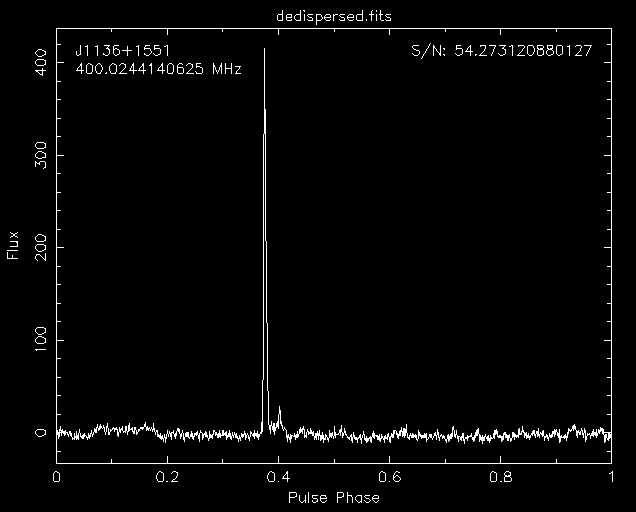
\includegraphics[width=0.45\textwidth]{Plots/dedispersed.png}
    \hspace{0.04\textwidth}
    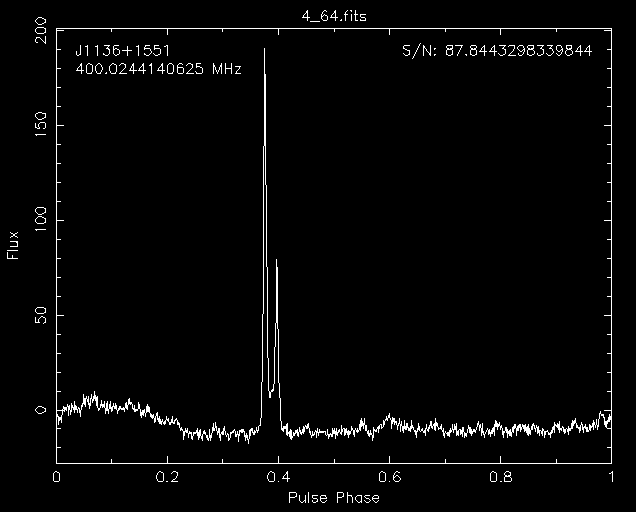
\includegraphics[width=0.45\textwidth]{Plots/4_64.png}
    \textbf{Figure 1:} Flux vs Phase, 1 subint \hspace*{3cm} \textbf{Figure 2:} Flux vs Phase, 4 subints
  \end{center}
\end{strip}

\begin{strip}
  \begin{center}
    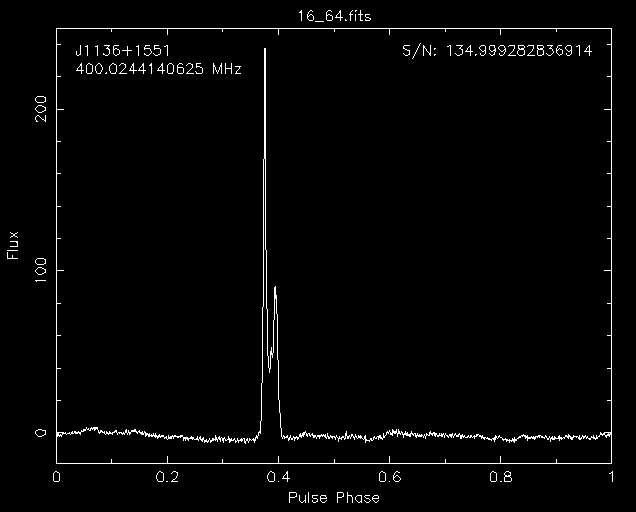
\includegraphics[width=0.45\textwidth]{Plots/16_64.png}    
    \hspace{0.04\textwidth}
    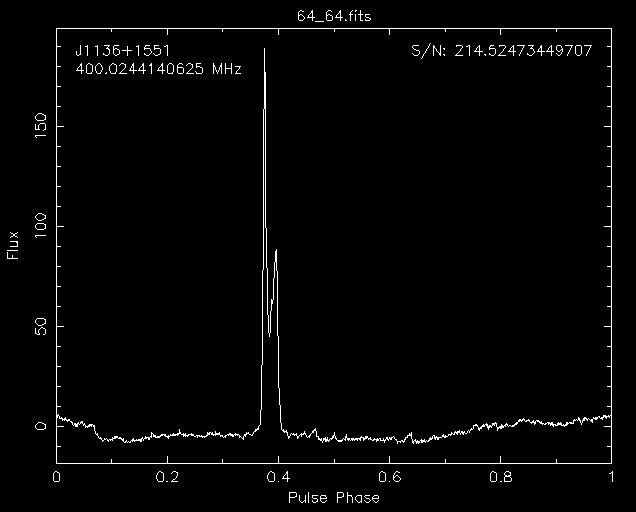
\includegraphics[width=0.45\textwidth]{Plots/64_64.png}
    \textbf{Figure 3:} Flux vs Phase, 16 subints \hspace*{2.5cm} \textbf{Figure 4:} Flux vs Phase, 64 subints
  \end{center}

  \vspace{4mm}
  \begin{center}
    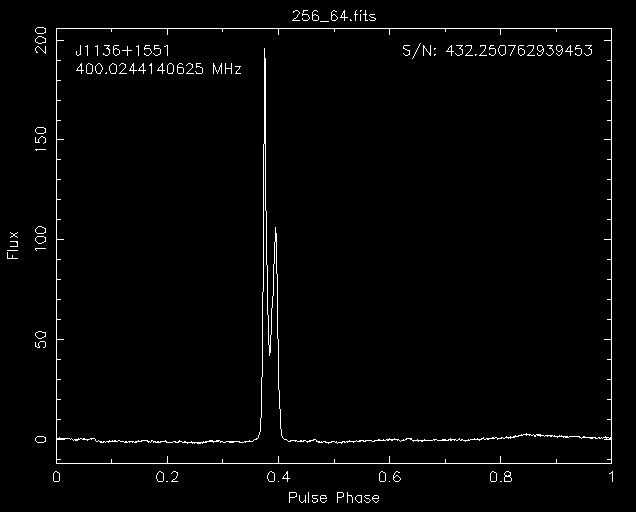
\includegraphics[width=0.45\textwidth]{Plots/256_64.png}
    \hspace{0.04\textwidth}
    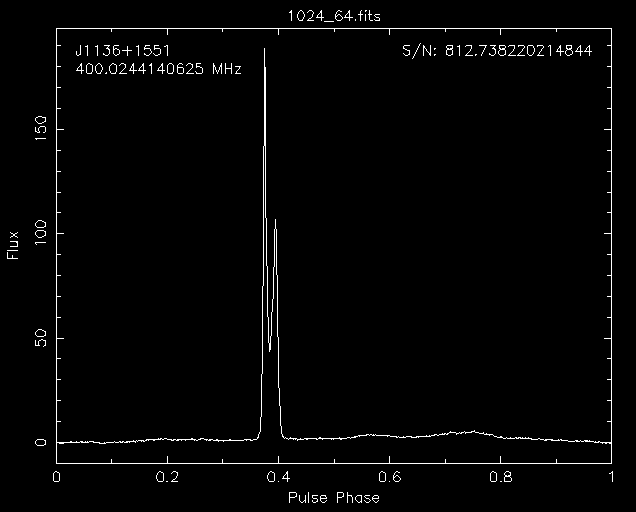
\includegraphics[width=0.45\textwidth]{Plots/1024_64.png}  
    \textbf{Figure 5:} Flux vs Phase, 256 subints \hspace*{2.5cm} \textbf{Figure 6:} Flux vs Phase, 802 subints
  \end{center}
\end{strip}

We can see that the pulse shape becomes more defined as we increase the integration time. This is because the signal gets averaged out over a longer period of time, which reduces the noise. This is also clear from the increase in the signal-to-noise ratio as we increase the integration time. We can plot the signal-to-noise ratio vs the number of subintegrations to see how it changes.

\begin{figure}[h!]
  \begin{center}
    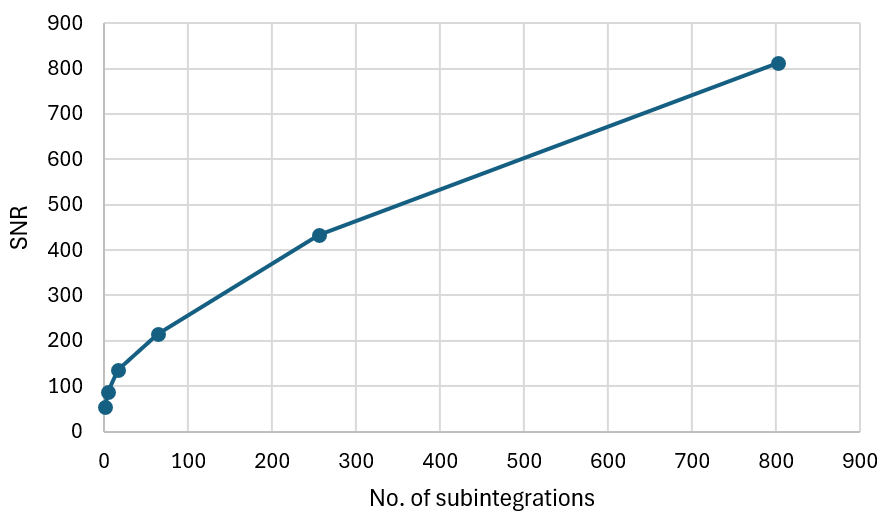
\includegraphics[width=0.8\columnwidth]{Plots/snr.png}
    \caption*{\textbf{Figure 7:} SNR vs No. of Subintegrations}
  \end{center}
\end{figure}


\subsubsection{pat}
Now that we have the different pulse profiles, we produce their time of arrival estimates. This requires the use of a template pulse profile. We can use the pulse profile obtained from integrating over the entire time period as the template as it has the highest signal-to-noise ratio. We can compare this with the other pulse profiles to get the time of arrival estimates. We store the template profile in \texttt{template.fits} and the pulsar profile to compare in \texttt{file.fits}. Then, we calculate the time of arrival by using the \texttt{pat} module:
\begin{verbatim}
  pat -s template.fits -f tempo2 file.fits
\end{verbatim}
The \texttt{-s} flag is used to declare the template file and the \texttt{-f} flag is used to provide the format of the output, which in this case is \texttt{tempo2}. Save the results obtained to a \texttt{.tim} file. 

We now have the frequency resolved time of arrivals for each pulse profile. These are used by the TEMPO2 software to calculate residuals, which give us information about the jitter present in the data.

\pagebreak
\subsection{TEMPO2}
TEMPO2 \cite{Edwards_2006} is a software used to analyse pulsar timing data. It can be used to calculate the residuals of the time of arrival estimates, which are the differences between the observed time of arrival and the predicted time of arrival. The residuals can be used to study the pulse jitter.

\subsubsection{Required components}
To calculate the residuals, we need to provide TEMPO2 with the timing estimates obtained from the \texttt{pat} module. We also need to provide it with the ephemeris of the pulsar. This is a set of parameters which describe the rotational and orbital behaviour of the pulsar. We can obtain the ephemeris from the ATNF Pulsar Catalogue. 

TEMPO2 uses the ephemeris file to create a model of the pulsar and calculate the expected time of arrival of the pulse. However, this model is not completely accurate since it does not account for pulse jitter. Thus, when we compare the expected time of arrival with the observed time of arrival, we get residuals. 

\subsubsection{Calculating residuals}
Once we have the ephemeris and the timing estimates, we can calculate the residuals and compare them over different integration times. We store the ephemeris in \texttt{parameter.par} and timing residuals in \texttt{timing.tim}. Then, we use the \texttt{tempo2} package:
\begin{verbatim}
  tempo2 -gr plk parameter.par timing.tim
\end{verbatim}

Running the above command starts the TEMPO2 interface. Here we can plot various characterisitics of the residuals. We can also use it to fit parameters related to the pulsar, like the frequency and the dispersion measure. 

\begin{figure}[h!]
  \begin{center}
    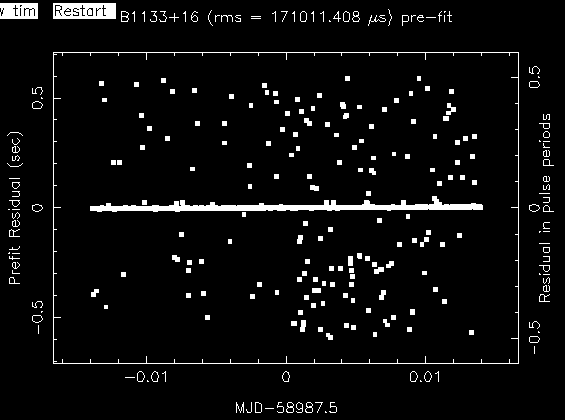
\includegraphics[width=0.9\columnwidth]{Plots/tempo1_edit.png}
    \caption*{\textbf{Figure 8:} Pre-fit Residuals vs Time, 1 subint}
  \end{center}
\end{figure}

We start by plotting the residuals of the original de-dispersed data against time. Notice above how there is a central high density line along with some outliers. These outliers represent the edge channels which have a higher noise level. The number of these outliers decreases as we increase the number of subintegrations. We can manually remove these from the interface to get a cleaner plot.

\begin{figure}[H]
  \begin{center}
    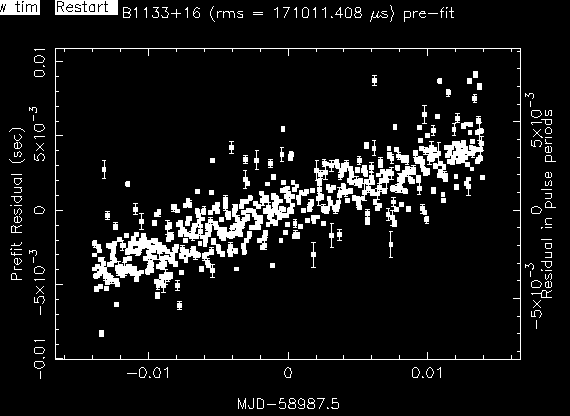
\includegraphics[width=0.9\columnwidth]{Plots/tempo2_edit.png}
    \caption*{\textbf{Figure 9:} Filtered pre-fit residuals vs Time, 1 subint}
  \end{center}
\end{figure}

We observe that the points are now in a straight line with a positive slope. This is caused by the slight difference in the time period between our data and the pular ephemeris. We can correct this by using \texttt{tempo2} to fit the frequency of the pulsar to the data. This should give us a straight line with a slope of 0.

\begin{figure}[H]
  \begin{center}
    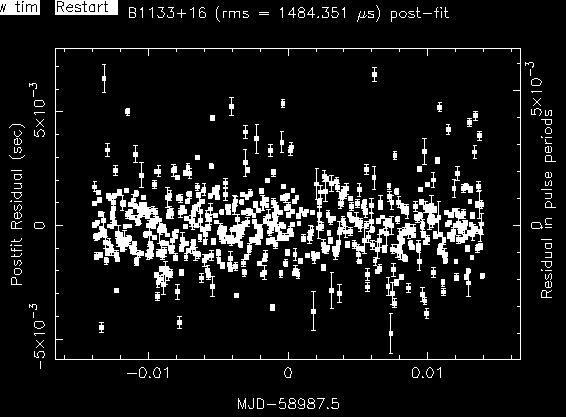
\includegraphics[width=0.9\columnwidth]{Plots/tempo3_edit.png}
    \caption*{\textbf{Figure 10:} Post-fit Residuals vs Time, 1 subint}
  \end{center}
\end{figure}

However, we see that the post-fit residuals do not form a straight line. They are scattered around the x axis. This is caused by the pulse jitter present in the data. The model used to fit the residuals does not account for the jitter, which results in residuals even after fitting the frequency.

We can repeat this experiment with the other pulse profiles to see how the residuals change with the integration time. The results obtained from this are shown below.

\begin{strip}
  \begin{center}
    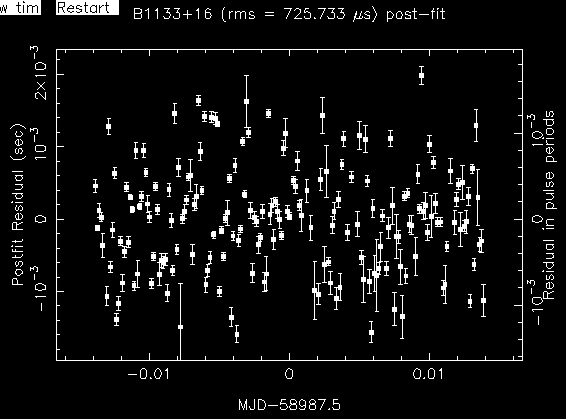
\includegraphics[width=0.45\textwidth]{Plots/tempo4_edit.png}
    \hspace{0.04\textwidth}
    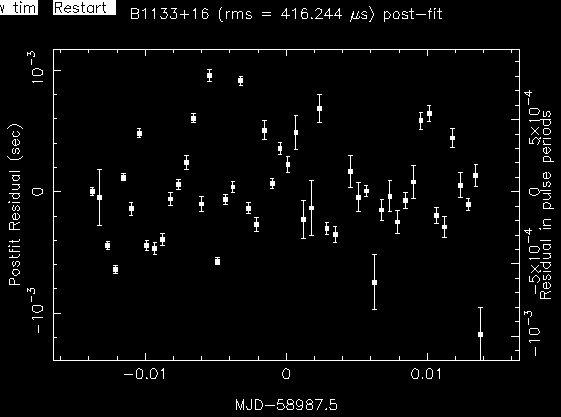
\includegraphics[width=0.45\textwidth]{Plots/tempo5_edit.png}
    \textbf{Figure 11:} Post-fit Residuals vs Time, 4 subints \hspace*{0.5cm} \textbf{Figure 12:} Post-fit Residuals vs Time, 16 subints
  \end{center}

  \vspace{4mm}
  \begin{center}
    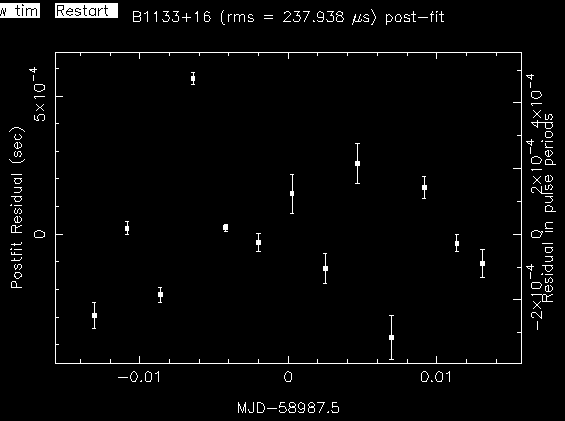
\includegraphics[width=0.45\textwidth]{Plots/tempo6_edit.png}    
    \hspace{0.04\textwidth}
    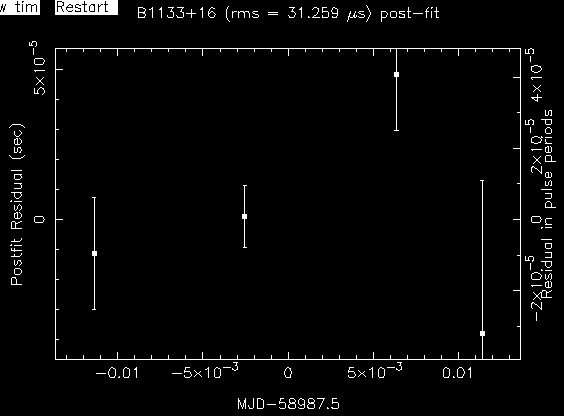
\includegraphics[width=0.45\textwidth]{Plots/tempo7_edit.png}
    \textbf{Figure 13:} Post-fit Residuals vs Time, 64 subints \hspace*{0.5cm} \textbf{Figure 14:} Post-fit Residuals vs Time, 256 subints
  \end{center}
\end{strip}

We can clearly see that the residuals decrease as we increase the integration time. This happens because our template file is just the average profile over the entire observation period. As we keep increasing the integration time, the pulse profile gets closer to the template profile, which reduces the residuals. 

\begin{figure}[h!]
  \begin{center}
    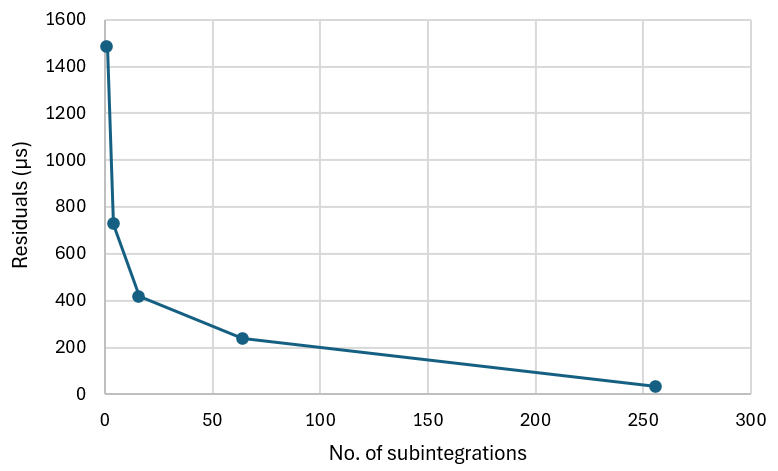
\includegraphics[width=0.85\columnwidth]{Plots/residuals.png}
    \caption*{\textbf{Figure 15:} Residuals vs No. of Subintegrations}
  \end{center}
\end{figure}

\vspace{2cm}
\section{RESULTS AND CONCLUSION}
We have confirmed the existence of pulse jitter and tried to quantify it through timing residuals. The shape of the pulsar is an important factor in determining its time of arrival. By plotting the flux vs phase for different integration times, we have seen how the pulse shape changes and how the signal-to-noise ratio increases with integration time. Thus increasing the integration time should also reduce the pulse jitter, which is confirmed by the residuals obtained from TEMPO2.

Our next goal should be to further quantify jitter and determine the factors which affect it. We can also investigate about the mechanism which causes jitter in pulsars. This would involve studying the physical structure of the pulsar and its magnetosphere. If we have a sufficient understanding of the cause of jitter, we can try to model it and account for it in our analysis. 
\clearpage

\nocite{burkesmith}
\nocite{lorimer}
\bibliographystyle{unsrt}
\bibliography{refs}

\end{document}
